% Options for packages loaded elsewhere
\PassOptionsToPackage{unicode}{hyperref}
\PassOptionsToPackage{hyphens}{url}
%
\documentclass[
]{article}
\usepackage{amsmath,amssymb}
\usepackage{lmodern}
\usepackage{ifxetex,ifluatex}
\ifnum 0\ifxetex 1\fi\ifluatex 1\fi=0 % if pdftex
  \usepackage[T1]{fontenc}
  \usepackage[utf8]{inputenc}
  \usepackage{textcomp} % provide euro and other symbols
\else % if luatex or xetex
  \usepackage{unicode-math}
  \defaultfontfeatures{Scale=MatchLowercase}
  \defaultfontfeatures[\rmfamily]{Ligatures=TeX,Scale=1}
\fi
% Use upquote if available, for straight quotes in verbatim environments
\IfFileExists{upquote.sty}{\usepackage{upquote}}{}
\IfFileExists{microtype.sty}{% use microtype if available
  \usepackage[]{microtype}
  \UseMicrotypeSet[protrusion]{basicmath} % disable protrusion for tt fonts
}{}
\makeatletter
\@ifundefined{KOMAClassName}{% if non-KOMA class
  \IfFileExists{parskip.sty}{%
    \usepackage{parskip}
  }{% else
    \setlength{\parindent}{0pt}
    \setlength{\parskip}{6pt plus 2pt minus 1pt}}
}{% if KOMA class
  \KOMAoptions{parskip=half}}
\makeatother
\usepackage{xcolor}
\IfFileExists{xurl.sty}{\usepackage{xurl}}{} % add URL line breaks if available
\IfFileExists{bookmark.sty}{\usepackage{bookmark}}{\usepackage{hyperref}}
\hypersetup{
  pdftitle={MATH 629 HW 3 Solutions},
  pdfauthor={Drew Lazar},
  hidelinks,
  pdfcreator={LaTeX via pandoc}}
\urlstyle{same} % disable monospaced font for URLs
\usepackage[margin=1in]{geometry}
\usepackage{color}
\usepackage{fancyvrb}
\newcommand{\VerbBar}{|}
\newcommand{\VERB}{\Verb[commandchars=\\\{\}]}
\DefineVerbatimEnvironment{Highlighting}{Verbatim}{commandchars=\\\{\}}
% Add ',fontsize=\small' for more characters per line
\usepackage{framed}
\definecolor{shadecolor}{RGB}{248,248,248}
\newenvironment{Shaded}{\begin{snugshade}}{\end{snugshade}}
\newcommand{\AlertTok}[1]{\textcolor[rgb]{0.94,0.16,0.16}{#1}}
\newcommand{\AnnotationTok}[1]{\textcolor[rgb]{0.56,0.35,0.01}{\textbf{\textit{#1}}}}
\newcommand{\AttributeTok}[1]{\textcolor[rgb]{0.77,0.63,0.00}{#1}}
\newcommand{\BaseNTok}[1]{\textcolor[rgb]{0.00,0.00,0.81}{#1}}
\newcommand{\BuiltInTok}[1]{#1}
\newcommand{\CharTok}[1]{\textcolor[rgb]{0.31,0.60,0.02}{#1}}
\newcommand{\CommentTok}[1]{\textcolor[rgb]{0.56,0.35,0.01}{\textit{#1}}}
\newcommand{\CommentVarTok}[1]{\textcolor[rgb]{0.56,0.35,0.01}{\textbf{\textit{#1}}}}
\newcommand{\ConstantTok}[1]{\textcolor[rgb]{0.00,0.00,0.00}{#1}}
\newcommand{\ControlFlowTok}[1]{\textcolor[rgb]{0.13,0.29,0.53}{\textbf{#1}}}
\newcommand{\DataTypeTok}[1]{\textcolor[rgb]{0.13,0.29,0.53}{#1}}
\newcommand{\DecValTok}[1]{\textcolor[rgb]{0.00,0.00,0.81}{#1}}
\newcommand{\DocumentationTok}[1]{\textcolor[rgb]{0.56,0.35,0.01}{\textbf{\textit{#1}}}}
\newcommand{\ErrorTok}[1]{\textcolor[rgb]{0.64,0.00,0.00}{\textbf{#1}}}
\newcommand{\ExtensionTok}[1]{#1}
\newcommand{\FloatTok}[1]{\textcolor[rgb]{0.00,0.00,0.81}{#1}}
\newcommand{\FunctionTok}[1]{\textcolor[rgb]{0.00,0.00,0.00}{#1}}
\newcommand{\ImportTok}[1]{#1}
\newcommand{\InformationTok}[1]{\textcolor[rgb]{0.56,0.35,0.01}{\textbf{\textit{#1}}}}
\newcommand{\KeywordTok}[1]{\textcolor[rgb]{0.13,0.29,0.53}{\textbf{#1}}}
\newcommand{\NormalTok}[1]{#1}
\newcommand{\OperatorTok}[1]{\textcolor[rgb]{0.81,0.36,0.00}{\textbf{#1}}}
\newcommand{\OtherTok}[1]{\textcolor[rgb]{0.56,0.35,0.01}{#1}}
\newcommand{\PreprocessorTok}[1]{\textcolor[rgb]{0.56,0.35,0.01}{\textit{#1}}}
\newcommand{\RegionMarkerTok}[1]{#1}
\newcommand{\SpecialCharTok}[1]{\textcolor[rgb]{0.00,0.00,0.00}{#1}}
\newcommand{\SpecialStringTok}[1]{\textcolor[rgb]{0.31,0.60,0.02}{#1}}
\newcommand{\StringTok}[1]{\textcolor[rgb]{0.31,0.60,0.02}{#1}}
\newcommand{\VariableTok}[1]{\textcolor[rgb]{0.00,0.00,0.00}{#1}}
\newcommand{\VerbatimStringTok}[1]{\textcolor[rgb]{0.31,0.60,0.02}{#1}}
\newcommand{\WarningTok}[1]{\textcolor[rgb]{0.56,0.35,0.01}{\textbf{\textit{#1}}}}
\usepackage{graphicx}
\makeatletter
\def\maxwidth{\ifdim\Gin@nat@width>\linewidth\linewidth\else\Gin@nat@width\fi}
\def\maxheight{\ifdim\Gin@nat@height>\textheight\textheight\else\Gin@nat@height\fi}
\makeatother
% Scale images if necessary, so that they will not overflow the page
% margins by default, and it is still possible to overwrite the defaults
% using explicit options in \includegraphics[width, height, ...]{}
\setkeys{Gin}{width=\maxwidth,height=\maxheight,keepaspectratio}
% Set default figure placement to htbp
\makeatletter
\def\fps@figure{htbp}
\makeatother
\setlength{\emergencystretch}{3em} % prevent overfull lines
\providecommand{\tightlist}{%
  \setlength{\itemsep}{0pt}\setlength{\parskip}{0pt}}
\setcounter{secnumdepth}{-\maxdimen} % remove section numbering
\ifluatex
  \usepackage{selnolig}  % disable illegal ligatures
\fi

\title{MATH 629 HW 3 Solutions}
\author{Drew Lazar}
\date{}

\begin{document}
\maketitle

\hypertarget{cleaning-up-and-loading-necessary-packages}{%
\subsection{Cleaning up and loading necessary
packages}\label{cleaning-up-and-loading-necessary-packages}}

\begin{Shaded}
\begin{Highlighting}[]
\FunctionTok{rm}\NormalTok{(}\AttributeTok{list=}\FunctionTok{ls}\NormalTok{())}
\FunctionTok{library}\NormalTok{(survival)}
\FunctionTok{library}\NormalTok{(dplyr)}
\end{Highlighting}
\end{Shaded}

\begin{verbatim}
## 
## Attaching package: 'dplyr'
\end{verbatim}

\begin{verbatim}
## The following objects are masked from 'package:stats':
## 
##     filter, lag
\end{verbatim}

\begin{verbatim}
## The following objects are masked from 'package:base':
## 
##     intersect, setdiff, setequal, union
\end{verbatim}

\hypertarget{i.-loading-the-data}{%
\subsection{1.i. loading the data}\label{i.-loading-the-data}}

\begin{Shaded}
\begin{Highlighting}[]
\FunctionTok{setwd}\NormalTok{(}\StringTok{"C:/GitStuff/Survival\_Analysis/MATH\_629/Data"}\NormalTok{)}
\NormalTok{Ven.reset }\OtherTok{\textless{}{-}}\FunctionTok{read.csv}\NormalTok{(}\StringTok{"Venreset.csv"}\NormalTok{, }\AttributeTok{header =} \ConstantTok{TRUE}\NormalTok{)}
\end{Highlighting}
\end{Shaded}

\hypertarget{create-a-survival-object-from-ventilator-data-set}{%
\subsection{2. create a survival object from Ventilator data
set}\label{create-a-survival-object-from-ventilator-data-set}}

\begin{Shaded}
\begin{Highlighting}[]
\NormalTok{Y}\OtherTok{\textless{}{-}}\FunctionTok{Surv}\NormalTok{(Ven.reset}\SpecialCharTok{$}\NormalTok{eventtime,Ven.reset}\SpecialCharTok{$}\NormalTok{status}\SpecialCharTok{==}\DecValTok{1}\NormalTok{)}
\end{Highlighting}
\end{Shaded}

\hypertarget{i.a.log-log-curves-for-setting}{%
\subsection{2.i.a.log-log curves for
Setting}\label{i.a.log-log-curves-for-setting}}

\begin{Shaded}
\begin{Highlighting}[]
\NormalTok{kmfitST3}\OtherTok{=}\FunctionTok{survfit}\NormalTok{(Y}\SpecialCharTok{\textasciitilde{}}\NormalTok{Ven.reset}\SpecialCharTok{$}\NormalTok{Setting)}
\FunctionTok{plot}\NormalTok{(kmfitST3,}\AttributeTok{fun=}\StringTok{"cloglog"}\NormalTok{,}\AttributeTok{xlab=}\StringTok{"time in days on log scale"}\NormalTok{,}\AttributeTok{ylab=}\StringTok{"log{-}log survival"}\NormalTok{, }\AttributeTok{main=}\StringTok{"log{-}log curves by Setting"}\NormalTok{,}\AttributeTok{col=}\FunctionTok{c}\NormalTok{(}\StringTok{\textquotesingle{}red\textquotesingle{}}\NormalTok{,}\StringTok{\textquotesingle{}green\textquotesingle{}}\NormalTok{,}\StringTok{\textquotesingle{}blue\textquotesingle{}}\NormalTok{))}
\FunctionTok{legend}\NormalTok{(}\StringTok{"topleft"}\NormalTok{,}\FunctionTok{c}\NormalTok{(}\StringTok{"Setting=2"}\NormalTok{,}\StringTok{"Setting=1"}\NormalTok{,}\StringTok{"Setting=0"}\NormalTok{),}\AttributeTok{lty=}\FunctionTok{c}\NormalTok{(}\StringTok{"solid"}\NormalTok{),}\AttributeTok{col=}\FunctionTok{c}\NormalTok{(}\StringTok{"red"}\NormalTok{,}\StringTok{"green"}\NormalTok{,}\StringTok{"blue"}\NormalTok{))}
\end{Highlighting}
\end{Shaded}

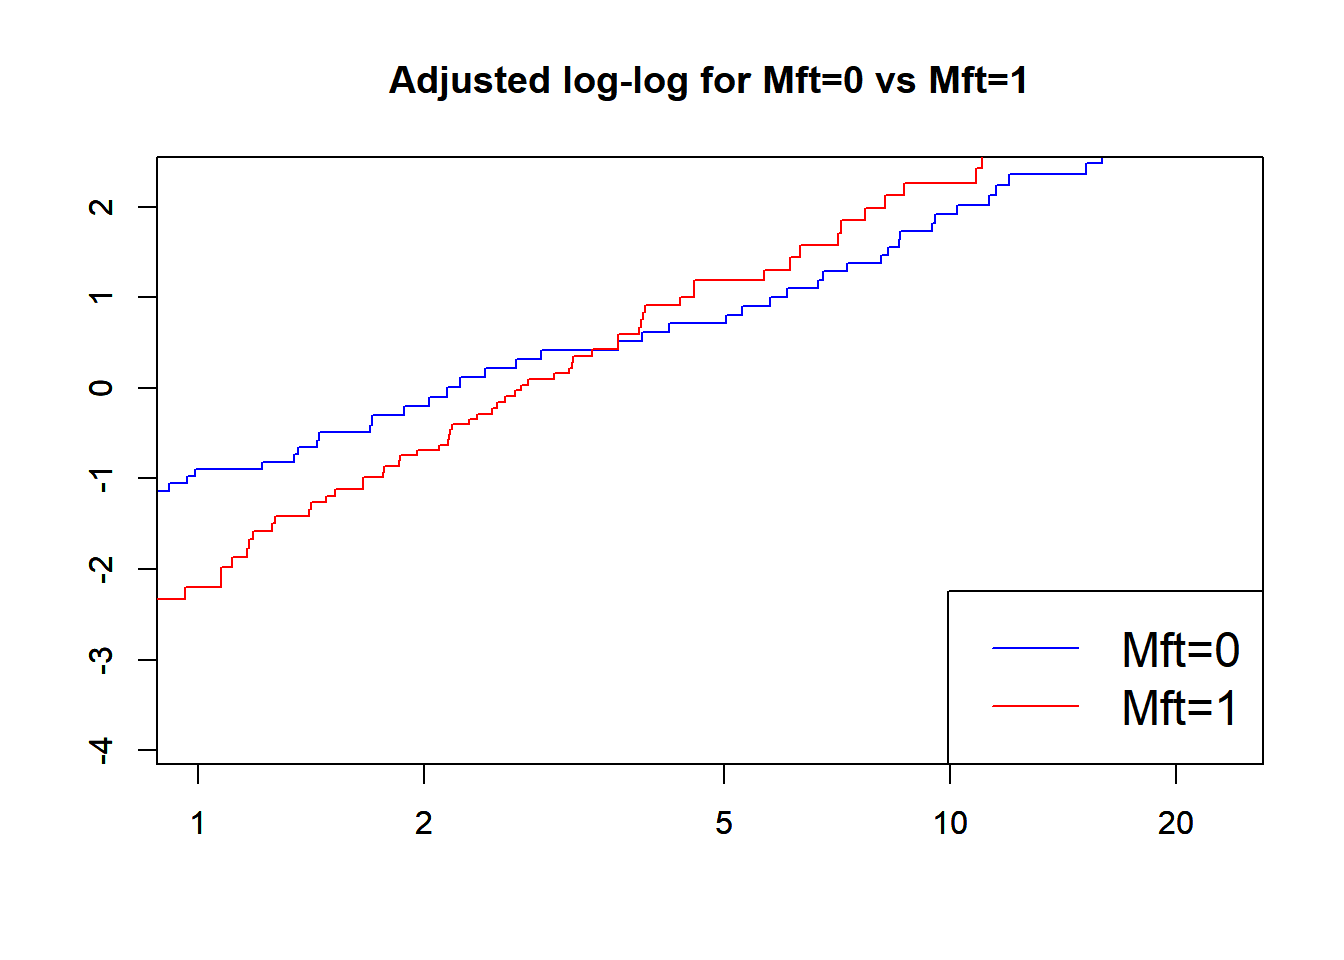
\includegraphics{HW3_629Solutions_files/figure-latex/unnamed-chunk-5-1.pdf}
\textbf{The log-log plots for Setting=0, Setting=1 and Setting=3 are
quite parallel throughout the study. There is some intersection at the
beginning of the study between Setting=2 and Setting=1 curves. This
intersection is exaggerated, however, due to the time axis being on the
log scale. Overall, the plots suggest that Setting satisfies the PH
assumption.}

\hypertarget{i.b.-log-log-curves-for-lo2}{%
\subsection{2.i.b. log-log curves for
LO2}\label{i.b.-log-log-curves-for-lo2}}

\begin{Shaded}
\begin{Highlighting}[]
\CommentTok{\#quantiles of LO2}
\FunctionTok{quantile}\NormalTok{(Ven.reset}\SpecialCharTok{$}\NormalTok{LO2)}
\end{Highlighting}
\end{Shaded}

\begin{verbatim}
##      0%     25%     50%     75%    100% 
## -2.5600  1.0075  2.0350  3.0825  6.2300
\end{verbatim}

\begin{Shaded}
\begin{Highlighting}[]
\NormalTok{Ven.reset}\SpecialCharTok{$}\NormalTok{LO2.group}\OtherTok{\textless{}{-}}\FunctionTok{cut}\NormalTok{(Ven.reset}\SpecialCharTok{$}\NormalTok{LO2,}\FunctionTok{c}\NormalTok{(}\SpecialCharTok{{-}}\FloatTok{2.58}\NormalTok{,}\FloatTok{1.0075}\NormalTok{,}\FloatTok{2.0350}\NormalTok{,}\FloatTok{3.0825}\NormalTok{,}\FloatTok{6.2300}\NormalTok{),}\AttributeTok{labels=}\FunctionTok{c}\NormalTok{(}\StringTok{\textquotesingle{}1\textquotesingle{}}\NormalTok{,}\StringTok{\textquotesingle{}2\textquotesingle{}}\NormalTok{,}\StringTok{\textquotesingle{}3\textquotesingle{}}\NormalTok{,}\StringTok{\textquotesingle{}4\textquotesingle{}}\NormalTok{))}
\end{Highlighting}
\end{Shaded}

\begin{Shaded}
\begin{Highlighting}[]
\NormalTok{kmfitO24}\OtherTok{=}\FunctionTok{survfit}\NormalTok{(Y}\SpecialCharTok{\textasciitilde{}}\NormalTok{Ven.reset}\SpecialCharTok{$}\NormalTok{LO2.group)}
\FunctionTok{plot}\NormalTok{(kmfitO24,}\AttributeTok{fun=}\StringTok{"cloglog"}\NormalTok{,}\AttributeTok{xlab=}\StringTok{"time in days on log scale"}\NormalTok{,}\AttributeTok{ylab=}\StringTok{"log{-}log survival"}\NormalTok{, }\AttributeTok{main=}\StringTok{"log{-}log curves by LO2group"}\NormalTok{,}\AttributeTok{col=}\FunctionTok{c}\NormalTok{(}\StringTok{"red"}\NormalTok{,}\StringTok{"green"}\NormalTok{,}\StringTok{"blue"}\NormalTok{,}\StringTok{"black"}\NormalTok{))}
\FunctionTok{legend}\NormalTok{(}\StringTok{"topleft"}\NormalTok{,}\AttributeTok{cex=}\NormalTok{.}\DecValTok{75}\NormalTok{,}\FunctionTok{c}\NormalTok{(}\StringTok{"LO2=high"}\NormalTok{,}\StringTok{"LO2=medhigh"}\NormalTok{,}\StringTok{"LO2=medlow"}\NormalTok{,}\StringTok{"LO2=low"}\NormalTok{),}\AttributeTok{lty=}\FunctionTok{c}\NormalTok{(}\StringTok{"solid"}\NormalTok{),}\AttributeTok{col=}\FunctionTok{c}\NormalTok{(}\StringTok{"red"}\NormalTok{,}\StringTok{"green"}\NormalTok{,}\StringTok{"blue"}\NormalTok{,}\StringTok{"black"}\NormalTok{))}
\end{Highlighting}
\end{Shaded}

\includegraphics{HW3_629Solutions_files/figure-latex/unnamed-chunk-7-1.pdf}
\textbf{The log-log plots are quite parallel which suggests that LO2 (as
stratified into LO2.group) satisfies the PH assumption. Note that the
log-log curves are at the same distance which suggests that the effect
of a change of LO2 on the survival experience is the same from low to
medlow, from medlow to medhigh and from medhigh to high.}

\hypertarget{ii.-alternative-approach-to-creating-log-log-plots-for-setting-assuming-statifies-ph-assumption.}{%
\subsection{2.ii. ``alternative'' approach to creating log-log plots for
Setting assuming \#\#statifies PH
assumption.}\label{ii.-alternative-approach-to-creating-log-log-plots-for-setting-assuming-statifies-ph-assumption.}}

\begin{Shaded}
\begin{Highlighting}[]
\CommentTok{\#Stratify Data set by Setting }
\NormalTok{Venreset0}\OtherTok{\textless{}{-}}\NormalTok{Ven.reset[Ven.reset}\SpecialCharTok{$}\NormalTok{Setting}\SpecialCharTok{==}\DecValTok{0}\NormalTok{, ]}
\NormalTok{Venreset1}\OtherTok{\textless{}{-}}\NormalTok{Ven.reset[Ven.reset}\SpecialCharTok{$}\NormalTok{Setting}\SpecialCharTok{==}\DecValTok{1}\NormalTok{, ]}
\NormalTok{Venreset2}\OtherTok{\textless{}{-}}\NormalTok{Ven.reset[Ven.reset}\SpecialCharTok{$}\NormalTok{Setting}\SpecialCharTok{==}\DecValTok{2}\NormalTok{, ]}
\CommentTok{\#Create Survival objects for three Strata}
\NormalTok{Y0}\OtherTok{\textless{}{-}}\FunctionTok{Surv}\NormalTok{(Venreset0}\SpecialCharTok{$}\NormalTok{eventtime,Venreset0}\SpecialCharTok{$}\NormalTok{status}\SpecialCharTok{==}\DecValTok{1}\NormalTok{)}
\NormalTok{Y1}\OtherTok{\textless{}{-}}\FunctionTok{Surv}\NormalTok{(Venreset1}\SpecialCharTok{$}\NormalTok{eventtime,Venreset1}\SpecialCharTok{$}\NormalTok{status}\SpecialCharTok{==}\DecValTok{1}\NormalTok{)}
\NormalTok{Y2}\OtherTok{\textless{}{-}}\FunctionTok{Surv}\NormalTok{(Venreset2}\SpecialCharTok{$}\NormalTok{eventtime,Venreset2}\SpecialCharTok{$}\NormalTok{status}\SpecialCharTok{==}\DecValTok{1}\NormalTok{)}
\CommentTok{\#Fit Cox PH models to three strata}
\NormalTok{Coxph.Ven.m0}\OtherTok{=}\FunctionTok{coxph}\NormalTok{(Y0}\SpecialCharTok{\textasciitilde{}}\NormalTok{LO2,}\AttributeTok{data=}\NormalTok{Venreset0)}
\NormalTok{Coxph.Ven.m1}\OtherTok{=}\FunctionTok{coxph}\NormalTok{(Y1}\SpecialCharTok{\textasciitilde{}}\NormalTok{LO2,}\AttributeTok{data=}\NormalTok{Venreset1)}
\NormalTok{Coxph.Ven.m2}\OtherTok{=}\FunctionTok{coxph}\NormalTok{(Y2}\SpecialCharTok{\textasciitilde{}}\NormalTok{LO2,}\AttributeTok{data=}\NormalTok{Venreset2)}
\CommentTok{\#get the overall mean of LO2}
\NormalTok{meanlo2}\OtherTok{=}\FunctionTok{mean}\NormalTok{(Ven.reset}\SpecialCharTok{$}\NormalTok{LO2)}
\end{Highlighting}
\end{Shaded}

\begin{Shaded}
\begin{Highlighting}[]
\CommentTok{\#plot our adjusted survival curves }
\NormalTok{pattern}\OtherTok{=}\FunctionTok{data.frame}\NormalTok{(}\AttributeTok{LO2=}\NormalTok{meanlo2)}
\FunctionTok{plot}\NormalTok{(}\AttributeTok{main=}\StringTok{"Adjusted log{-}log survival curves for Setting w/mean(LO2)"}\NormalTok{,}\FunctionTok{survfit}\NormalTok{(Coxph.Ven.m0,}\AttributeTok{newdata=}\NormalTok{pattern),}\AttributeTok{xlim=}\FunctionTok{c}\NormalTok{(}\FloatTok{0.08}\NormalTok{,}\DecValTok{23}\NormalTok{),}\AttributeTok{ylim=}\FunctionTok{c}\NormalTok{(}\SpecialCharTok{{-}}\DecValTok{6}\NormalTok{,}\FloatTok{3.7}\NormalTok{),}\AttributeTok{fun=}\StringTok{"cloglog"}\NormalTok{,}\AttributeTok{conf.int=}\NormalTok{F,}\AttributeTok{col=}\FunctionTok{c}\NormalTok{(}\StringTok{\textquotesingle{}blue\textquotesingle{}}\NormalTok{))}
\FunctionTok{par}\NormalTok{(}\AttributeTok{new=}\ConstantTok{TRUE}\NormalTok{)}
\FunctionTok{plot}\NormalTok{(}\FunctionTok{survfit}\NormalTok{(Coxph.Ven.m1,}\AttributeTok{newdata=}\NormalTok{pattern),}\AttributeTok{xlim=}\FunctionTok{c}\NormalTok{(}\FloatTok{0.08}\NormalTok{,}\DecValTok{23}\NormalTok{),}\AttributeTok{ylim=}\FunctionTok{c}\NormalTok{(}\SpecialCharTok{{-}}\DecValTok{6}\NormalTok{,}\FloatTok{3.7}\NormalTok{),}\AttributeTok{fun=}\StringTok{"cloglog"}\NormalTok{,}\AttributeTok{conf.int=}\NormalTok{F,}\AttributeTok{col=}\NormalTok{(}\StringTok{\textquotesingle{}green\textquotesingle{}}\NormalTok{))}
\FunctionTok{par}\NormalTok{(}\AttributeTok{new=}\ConstantTok{TRUE}\NormalTok{)}
\FunctionTok{plot}\NormalTok{(}\FunctionTok{survfit}\NormalTok{(Coxph.Ven.m2,}\AttributeTok{newdata=}\NormalTok{pattern),}\AttributeTok{fun=}\StringTok{"cloglog"}\NormalTok{,}\AttributeTok{xlim=}\FunctionTok{c}\NormalTok{(}\FloatTok{0.08}\NormalTok{,}\DecValTok{23}\NormalTok{),}\AttributeTok{ylim=}\FunctionTok{c}\NormalTok{(}\SpecialCharTok{{-}}\DecValTok{6}\NormalTok{,}\FloatTok{3.7}\NormalTok{),}\AttributeTok{conf.int=}\NormalTok{F,}\AttributeTok{col=}\NormalTok{(}\StringTok{\textquotesingle{}red\textquotesingle{}}\NormalTok{))}
\FunctionTok{legend}\NormalTok{(}\StringTok{"topleft"}\NormalTok{,}\FunctionTok{c}\NormalTok{(}\StringTok{"Setting=0"}\NormalTok{,}\StringTok{"Setting=1"}\NormalTok{,}\StringTok{"Setting=2"}\NormalTok{),}\AttributeTok{lty=}\NormalTok{(}\StringTok{\textquotesingle{}solid\textquotesingle{}}\NormalTok{),}\AttributeTok{col=}\FunctionTok{c}\NormalTok{(}\StringTok{\textquotesingle{}red\textquotesingle{}}\NormalTok{,}\StringTok{\textquotesingle{}green\textquotesingle{}}\NormalTok{,}\StringTok{\textquotesingle{}blue\textquotesingle{}}\NormalTok{))}
\end{Highlighting}
\end{Shaded}

\includegraphics{HW3_629Solutions_files/figure-latex/unnamed-chunk-9-1.pdf}
\textbf{This plot differs from the plot created in 2.i.a. in that these
curves cross a bit less significantly than the log-log survival curves
created in 2.i.a. This suggests some interaction of LO2 with Setting as
Setting seems to satisfy the PH assumption to a bit more of an extent
while considering LO2. }

\hypertarget{observed-vs.-expected-plots}{%
\subsection{3. Observed vs.~Expected
Plots}\label{observed-vs.-expected-plots}}

\hypertarget{i.-observed-vs.-expected-plots-for-setting}{%
\subsection{3i. Observed vs.~Expected plots for
Setting}\label{i.-observed-vs.-expected-plots-for-setting}}

\begin{Shaded}
\begin{Highlighting}[]
\CommentTok{\#fit a Cox PH model against setting }
\NormalTok{Coxph.Ven.Setting}\OtherTok{=}\FunctionTok{coxph}\NormalTok{(Y}\SpecialCharTok{\textasciitilde{}}\NormalTok{Setting,}\AttributeTok{data=}\NormalTok{Ven.reset)}
\NormalTok{pattern1}\OtherTok{=}\FunctionTok{data.frame}\NormalTok{(}\AttributeTok{Setting=}\DecValTok{0}\NormalTok{)}
\NormalTok{pattern2}\OtherTok{=}\FunctionTok{data.frame}\NormalTok{(}\AttributeTok{Setting=}\DecValTok{1}\NormalTok{)}
\NormalTok{pattern3}\OtherTok{=}\FunctionTok{data.frame}\NormalTok{(}\AttributeTok{Setting=}\DecValTok{2}\NormalTok{)}
\end{Highlighting}
\end{Shaded}

\begin{Shaded}
\begin{Highlighting}[]
\CommentTok{\#Plot our Expected Curves}
\FunctionTok{plot}\NormalTok{(kmfitST3,}\AttributeTok{main=}\StringTok{"Observed vs Expected curves by Setting"}\NormalTok{,}\AttributeTok{xlab=}\StringTok{"time in days"}\NormalTok{,}\AttributeTok{ylab=}\StringTok{"Survival Probabilities"}\NormalTok{, }\AttributeTok{col=}\FunctionTok{c}\NormalTok{(}\StringTok{\textquotesingle{}blue\textquotesingle{}}\NormalTok{,}\StringTok{\textquotesingle{}green\textquotesingle{}}\NormalTok{,}\StringTok{\textquotesingle{}red\textquotesingle{}}\NormalTok{),}\AttributeTok{lty=}\FunctionTok{c}\NormalTok{(}\StringTok{\textquotesingle{}solid\textquotesingle{}}\NormalTok{,}\StringTok{\textquotesingle{}solid\textquotesingle{}}\NormalTok{,}\StringTok{\textquotesingle{}solid\textquotesingle{}}\NormalTok{))}
\CommentTok{\#Plot our Observed Curves for each setting }
\FunctionTok{par}\NormalTok{(}\AttributeTok{new=}\ConstantTok{TRUE}\NormalTok{)}
\FunctionTok{plot}\NormalTok{(}\FunctionTok{survfit}\NormalTok{(Coxph.Ven.Setting,}\AttributeTok{newdata=}\NormalTok{pattern1),}\AttributeTok{conf.int=}\NormalTok{F,}\AttributeTok{col=}\FunctionTok{c}\NormalTok{(}\StringTok{\textquotesingle{}blue\textquotesingle{}}\NormalTok{),}\AttributeTok{lty=}\FunctionTok{c}\NormalTok{(}\StringTok{\textquotesingle{}dashed\textquotesingle{}}\NormalTok{))}
\FunctionTok{par}\NormalTok{(}\AttributeTok{new=}\ConstantTok{TRUE}\NormalTok{)}
\FunctionTok{plot}\NormalTok{(}\FunctionTok{survfit}\NormalTok{(Coxph.Ven.Setting,}\AttributeTok{newdata=}\NormalTok{pattern2),}\AttributeTok{conf.int=}\NormalTok{F,}\AttributeTok{col=}\FunctionTok{c}\NormalTok{(}\StringTok{\textquotesingle{}green\textquotesingle{}}\NormalTok{),}\AttributeTok{lty=}\FunctionTok{c}\NormalTok{(}\StringTok{\textquotesingle{}dashed\textquotesingle{}}\NormalTok{))}
\FunctionTok{par}\NormalTok{(}\AttributeTok{new=}\ConstantTok{TRUE}\NormalTok{)}
\FunctionTok{plot}\NormalTok{(}\FunctionTok{survfit}\NormalTok{(Coxph.Ven.Setting,}\AttributeTok{newdata=}\NormalTok{pattern3),}\AttributeTok{conf.int=}\NormalTok{F,}\AttributeTok{col=}\FunctionTok{c}\NormalTok{(}\StringTok{\textquotesingle{}red\textquotesingle{}}\NormalTok{),}\AttributeTok{lty=}\FunctionTok{c}\NormalTok{(}\StringTok{\textquotesingle{}dashed\textquotesingle{}}\NormalTok{))}
\FunctionTok{legend}\NormalTok{(}\StringTok{"topright"}\NormalTok{,}\FunctionTok{c}\NormalTok{(}\StringTok{"Setting=0(observed)"}\NormalTok{,}\StringTok{"Setting=1(observed)"}\NormalTok{,}\StringTok{"Setting=2(observed)"}\NormalTok{,}\StringTok{"Setting=0(expected)"}\NormalTok{,}\StringTok{"Setting=1(expected)"}\NormalTok{,}\StringTok{"Setting=2(expected)"}\NormalTok{),}\AttributeTok{lty=}\FunctionTok{c}\NormalTok{(}\StringTok{\textquotesingle{}solid\textquotesingle{}}\NormalTok{,}\StringTok{\textquotesingle{}solid\textquotesingle{}}\NormalTok{,}\StringTok{\textquotesingle{}solid\textquotesingle{}}\NormalTok{,}\StringTok{\textquotesingle{}dashed\textquotesingle{}}\NormalTok{,}\StringTok{\textquotesingle{}dashed\textquotesingle{}}\NormalTok{,}\StringTok{\textquotesingle{}dashed\textquotesingle{}}\NormalTok{),}\AttributeTok{col=}\FunctionTok{c}\NormalTok{(}\StringTok{\textquotesingle{}blue\textquotesingle{}}\NormalTok{,}\StringTok{\textquotesingle{}green\textquotesingle{}}\NormalTok{,}\StringTok{\textquotesingle{}red\textquotesingle{}}\NormalTok{,}\StringTok{\textquotesingle{}blue\textquotesingle{}}\NormalTok{,}\StringTok{\textquotesingle{}green\textquotesingle{}}\NormalTok{,}\StringTok{\textquotesingle{}red\textquotesingle{}}\NormalTok{))}
\end{Highlighting}
\end{Shaded}

\includegraphics{HW3_629Solutions_files/figure-latex/unnamed-chunk-11-1.pdf}
\textbf{As the observed vs.~expected plots are similar these plots
suggest that the Cox PH assumption is met for Setting} \#\# 3.ii.
Observed vs.~Expected plots for LO2

\hypertarget{ii.a.-expected-are-adjusted-survival-curves-using-mean-in-each-strata}{%
\subsection{3.ii.a. Expected are adjusted survival curves using mean in
each
strata}\label{ii.a.-expected-are-adjusted-survival-curves-using-mean-in-each-strata}}

\begin{Shaded}
\begin{Highlighting}[]
\CommentTok{\#Get mean in each strata }
\NormalTok{Ven.reset }\SpecialCharTok{\%\textgreater{}\%}
  \FunctionTok{group\_by}\NormalTok{(LO2.group) }\SpecialCharTok{\%\textgreater{}\%}
  \FunctionTok{summarise}\NormalTok{(}\AttributeTok{mean\_LO2 =} \FunctionTok{mean}\NormalTok{(LO2))}
\end{Highlighting}
\end{Shaded}

\begin{verbatim}
## # A tibble: 4 x 2
##   LO2.group mean_LO2
##   <fct>        <dbl>
## 1 1           -0.421
## 2 2            1.45 
## 3 3            2.44 
## 4 4            4.01
\end{verbatim}

\begin{Shaded}
\begin{Highlighting}[]
\NormalTok{Coxph.Ven.LO2}\OtherTok{=}\FunctionTok{coxph}\NormalTok{(Y}\SpecialCharTok{\textasciitilde{}}\NormalTok{LO2,}\AttributeTok{data=}\NormalTok{Ven.reset)}
\NormalTok{pattern1}\OtherTok{=}\FunctionTok{data.frame}\NormalTok{(}\AttributeTok{LO2=}\SpecialCharTok{{-}}\FloatTok{0.421}\NormalTok{)}
\NormalTok{pattern2}\OtherTok{=}\FunctionTok{data.frame}\NormalTok{(}\AttributeTok{LO2=}\FloatTok{1.456}\NormalTok{)}
\NormalTok{pattern3}\OtherTok{=}\FunctionTok{data.frame}\NormalTok{(}\AttributeTok{LO2=}\FloatTok{2.439}\NormalTok{)}
\NormalTok{pattern4}\OtherTok{=}\FunctionTok{data.frame}\NormalTok{(}\AttributeTok{LO2=}\FloatTok{4.011}\NormalTok{)}
\end{Highlighting}
\end{Shaded}

\begin{Shaded}
\begin{Highlighting}[]
\CommentTok{\#Plot expected curves}
\FunctionTok{plot}\NormalTok{(kmfitO24,}\AttributeTok{xlab=}\StringTok{"time in weeks on log scale"}\NormalTok{,}\AttributeTok{ylab=}\StringTok{"Survival Probabilities"}\NormalTok{, }\AttributeTok{col=}\FunctionTok{c}\NormalTok{(}\StringTok{\textquotesingle{}blue\textquotesingle{}}\NormalTok{,}\StringTok{\textquotesingle{}green\textquotesingle{}}\NormalTok{,}\StringTok{\textquotesingle{}red\textquotesingle{}}\NormalTok{,}\StringTok{\textquotesingle{}blueviolet\textquotesingle{}}\NormalTok{), }\AttributeTok{main=}\StringTok{"Observed vs. Expected by level of LO2"}\NormalTok{)}
\CommentTok{\#Plot observed curves}
\FunctionTok{par}\NormalTok{(}\AttributeTok{new=}\ConstantTok{TRUE}\NormalTok{)}
\FunctionTok{plot}\NormalTok{(}\FunctionTok{survfit}\NormalTok{(Coxph.Ven.LO2,}\AttributeTok{newdata=}\NormalTok{pattern1),}\AttributeTok{conf.int=}\NormalTok{F,}\AttributeTok{col=}\FunctionTok{c}\NormalTok{(}\StringTok{\textquotesingle{}blue\textquotesingle{}}\NormalTok{),}\AttributeTok{lty=}\FunctionTok{c}\NormalTok{(}\StringTok{\textquotesingle{}dashed\textquotesingle{}}\NormalTok{))}
\FunctionTok{par}\NormalTok{(}\AttributeTok{new=}\ConstantTok{TRUE}\NormalTok{)  }
\FunctionTok{plot}\NormalTok{(}\FunctionTok{survfit}\NormalTok{(Coxph.Ven.LO2,}\AttributeTok{newdata=}\NormalTok{pattern2),}\AttributeTok{conf.int=}\NormalTok{F,}\AttributeTok{col=}\FunctionTok{c}\NormalTok{(}\StringTok{\textquotesingle{}green\textquotesingle{}}\NormalTok{),}\AttributeTok{lty=}\FunctionTok{c}\NormalTok{(}\StringTok{\textquotesingle{}dashed\textquotesingle{}}\NormalTok{))}
\FunctionTok{par}\NormalTok{(}\AttributeTok{new=}\ConstantTok{TRUE}\NormalTok{)}
\FunctionTok{plot}\NormalTok{(}\FunctionTok{survfit}\NormalTok{(Coxph.Ven.LO2,}\AttributeTok{newdata=}\NormalTok{pattern3),}\AttributeTok{conf.int=}\NormalTok{F,}\AttributeTok{col=}\FunctionTok{c}\NormalTok{(}\StringTok{\textquotesingle{}red\textquotesingle{}}\NormalTok{),}\AttributeTok{lty=}\FunctionTok{c}\NormalTok{(}\StringTok{\textquotesingle{}dashed\textquotesingle{}}\NormalTok{))}
\FunctionTok{par}\NormalTok{(}\AttributeTok{new=}\ConstantTok{TRUE}\NormalTok{)}
\FunctionTok{plot}\NormalTok{(}\FunctionTok{survfit}\NormalTok{(Coxph.Ven.LO2,}\AttributeTok{newdata=}\NormalTok{pattern4),}\AttributeTok{conf.int=}\NormalTok{F,}\AttributeTok{col=}\FunctionTok{c}\NormalTok{(}\StringTok{\textquotesingle{}blueviolet\textquotesingle{}}\NormalTok{),}\AttributeTok{lty=}\FunctionTok{c}\NormalTok{(}\StringTok{\textquotesingle{}dashed\textquotesingle{}}\NormalTok{))}
\FunctionTok{legend}\NormalTok{(}\StringTok{"topright"}\NormalTok{,}\AttributeTok{cex=}\NormalTok{.}\DecValTok{75}\NormalTok{,}\FunctionTok{c}\NormalTok{(}\StringTok{"LO2=low (observed)"}\NormalTok{,}\StringTok{"LO2=medlow (observed)"}\NormalTok{,}\StringTok{"LO2=medhigh (observed)"}\NormalTok{,}\StringTok{"LO2=high (observed)"}\NormalTok{,}\StringTok{"LO2=low (expected)"}\NormalTok{,}\StringTok{"LO2=medlow (expected)"}\NormalTok{,}\StringTok{"LO2=medhigh (expected)"}\NormalTok{,}\StringTok{"LO2=high (expected)"}\NormalTok{),}\AttributeTok{lty=}\FunctionTok{cbind}\NormalTok{(}\FunctionTok{rep}\NormalTok{(}\StringTok{\textquotesingle{}solid\textquotesingle{}}\NormalTok{,}\DecValTok{4}\NormalTok{),}\FunctionTok{rep}\NormalTok{(}\StringTok{\textquotesingle{}dashed\textquotesingle{}}\NormalTok{,}\DecValTok{4}\NormalTok{)),}\AttributeTok{col=}\FunctionTok{rep}\NormalTok{(}\FunctionTok{c}\NormalTok{(}\StringTok{\textquotesingle{}blue\textquotesingle{}}\NormalTok{,}\StringTok{\textquotesingle{}red\textquotesingle{}}\NormalTok{,}\StringTok{\textquotesingle{}green\textquotesingle{}}\NormalTok{,}\StringTok{\textquotesingle{}blueviolet\textquotesingle{}}\NormalTok{),}\DecValTok{2}\NormalTok{)) }
\end{Highlighting}
\end{Shaded}

\includegraphics{HW3_629Solutions_files/figure-latex/unnamed-chunk-13-1.pdf}
\textbf{These plots suggest that LO2 satisfies the PH assumption.}

\#\#3.ii.b. Expected adjusted survival curves using dummy variables

\begin{Shaded}
\begin{Highlighting}[]
\CommentTok{\#Create dummy variables and fit Cox PH model against dummy variables }
\NormalTok{Ven.reset}\SpecialCharTok{$}\NormalTok{X1}\OtherTok{\textless{}{-}}\FunctionTok{rep}\NormalTok{(}\DecValTok{0}\NormalTok{,}\FunctionTok{nrow}\NormalTok{(Ven.reset));Ven.reset}\SpecialCharTok{$}\NormalTok{X2}\OtherTok{\textless{}{-}}\FunctionTok{rep}\NormalTok{(}\DecValTok{0}\NormalTok{,}\FunctionTok{nrow}\NormalTok{(Ven.reset))}
\NormalTok{Ven.reset}\SpecialCharTok{$}\NormalTok{X3}\OtherTok{\textless{}{-}}\FunctionTok{rep}\NormalTok{(}\DecValTok{0}\NormalTok{,}\FunctionTok{nrow}\NormalTok{(Ven.reset))}
\ControlFlowTok{for}\NormalTok{ (i }\ControlFlowTok{in} \DecValTok{1}\SpecialCharTok{:}\FunctionTok{nrow}\NormalTok{(Ven.reset))}
\NormalTok{\{}
  \ControlFlowTok{if}\NormalTok{ (Ven.reset}\SpecialCharTok{$}\NormalTok{LO2.group[i] }\SpecialCharTok{==} \DecValTok{2}\NormalTok{) \{}
\NormalTok{    Ven.reset}\SpecialCharTok{$}\NormalTok{X1[i]}\OtherTok{=}\DecValTok{1}
\NormalTok{  \} }\ControlFlowTok{else} \ControlFlowTok{if}\NormalTok{ (Ven.reset}\SpecialCharTok{$}\NormalTok{LO2.group[i]}\SpecialCharTok{==}\DecValTok{3}\NormalTok{) \{}
\NormalTok{    Ven.reset}\SpecialCharTok{$}\NormalTok{X2[i]}\OtherTok{=}\DecValTok{1} 
\NormalTok{  \} }\ControlFlowTok{else} \ControlFlowTok{if}\NormalTok{ (Ven.reset}\SpecialCharTok{$}\NormalTok{LO2.group[i]}\SpecialCharTok{==}\DecValTok{4}\NormalTok{) \{}
\NormalTok{    Ven.reset}\SpecialCharTok{$}\NormalTok{X3[i]}\OtherTok{=}\DecValTok{1} 
\NormalTok{  \}}
\NormalTok{\}}
\NormalTok{Coxph.Ven.LO2.d}\OtherTok{=}\FunctionTok{coxph}\NormalTok{(Y}\SpecialCharTok{\textasciitilde{}}\NormalTok{X1}\SpecialCharTok{+}\NormalTok{X2}\SpecialCharTok{+}\NormalTok{X3,}\AttributeTok{data=}\NormalTok{Ven.reset)}
\NormalTok{Coxph.Ven.LO2.g}\OtherTok{=}\FunctionTok{coxph}\NormalTok{(Y}\SpecialCharTok{\textasciitilde{}}\NormalTok{LO2.group,Ven.reset)}
\NormalTok{pattern1}\OtherTok{=}\FunctionTok{data.frame}\NormalTok{(}\AttributeTok{X1=}\DecValTok{0}\NormalTok{,}\AttributeTok{X2=}\DecValTok{0}\NormalTok{,}\AttributeTok{X3=}\DecValTok{0}\NormalTok{)}
\NormalTok{pattern2}\OtherTok{=}\FunctionTok{data.frame}\NormalTok{(}\AttributeTok{X1=}\DecValTok{1}\NormalTok{,}\AttributeTok{X2=}\DecValTok{0}\NormalTok{,}\AttributeTok{X3=}\DecValTok{0}\NormalTok{)}
\NormalTok{pattern3}\OtherTok{=}\FunctionTok{data.frame}\NormalTok{(}\AttributeTok{X1=}\DecValTok{0}\NormalTok{,}\AttributeTok{X2=}\DecValTok{1}\NormalTok{,}\AttributeTok{X3=}\DecValTok{0}\NormalTok{)}
\NormalTok{pattern4}\OtherTok{=}\FunctionTok{data.frame}\NormalTok{(}\AttributeTok{X1=}\DecValTok{0}\NormalTok{,}\AttributeTok{X2=}\DecValTok{0}\NormalTok{,}\AttributeTok{X3=}\DecValTok{1}\NormalTok{)}
\end{Highlighting}
\end{Shaded}

\begin{Shaded}
\begin{Highlighting}[]
\CommentTok{\#Plot expected curves }
\FunctionTok{plot}\NormalTok{(kmfitO24,}\AttributeTok{xlab=}\StringTok{"time in weeks on log scale"}\NormalTok{,}\AttributeTok{ylab=}\StringTok{"Survival Probabilities"}\NormalTok{, }\AttributeTok{col=}\FunctionTok{c}\NormalTok{(}\StringTok{\textquotesingle{}blue\textquotesingle{}}\NormalTok{,}\StringTok{\textquotesingle{}green\textquotesingle{}}\NormalTok{,}\StringTok{\textquotesingle{}red\textquotesingle{}}\NormalTok{,}\StringTok{\textquotesingle{}blueviolet\textquotesingle{}}\NormalTok{), }\AttributeTok{main=}\StringTok{"Observed vs. Expected by level of LogWBC"}\NormalTok{)}
\CommentTok{\#Plot adjusted survival curves}
\FunctionTok{par}\NormalTok{(}\AttributeTok{new=}\ConstantTok{TRUE}\NormalTok{)}
\FunctionTok{plot}\NormalTok{(}\FunctionTok{survfit}\NormalTok{(Coxph.Ven.LO2.d,}\AttributeTok{newdata=}\NormalTok{pattern1),}\AttributeTok{conf.int=}\NormalTok{F,}\AttributeTok{col=}\FunctionTok{c}\NormalTok{(}\StringTok{\textquotesingle{}blue\textquotesingle{}}\NormalTok{),}\AttributeTok{lty=}\FunctionTok{c}\NormalTok{(}\StringTok{\textquotesingle{}dashed\textquotesingle{}}\NormalTok{))}
\FunctionTok{par}\NormalTok{(}\AttributeTok{new=}\ConstantTok{TRUE}\NormalTok{)  }
\FunctionTok{plot}\NormalTok{(}\FunctionTok{survfit}\NormalTok{(Coxph.Ven.LO2.d,}\AttributeTok{newdata=}\NormalTok{pattern2),}\AttributeTok{conf.int=}\NormalTok{F,}\AttributeTok{col=}\FunctionTok{c}\NormalTok{(}\StringTok{\textquotesingle{}green\textquotesingle{}}\NormalTok{),}\AttributeTok{lty=}\FunctionTok{c}\NormalTok{(}\StringTok{\textquotesingle{}dashed\textquotesingle{}}\NormalTok{))}
\FunctionTok{par}\NormalTok{(}\AttributeTok{new=}\ConstantTok{TRUE}\NormalTok{)}
\FunctionTok{plot}\NormalTok{(}\FunctionTok{survfit}\NormalTok{(Coxph.Ven.LO2.d,}\AttributeTok{newdata=}\NormalTok{pattern3),}\AttributeTok{conf.int=}\NormalTok{F,}\AttributeTok{col=}\FunctionTok{c}\NormalTok{(}\StringTok{\textquotesingle{}red\textquotesingle{}}\NormalTok{),}\AttributeTok{lty=}\FunctionTok{c}\NormalTok{(}\StringTok{\textquotesingle{}dashed\textquotesingle{}}\NormalTok{))}
\FunctionTok{par}\NormalTok{(}\AttributeTok{new=}\ConstantTok{TRUE}\NormalTok{)}
\FunctionTok{plot}\NormalTok{(}\FunctionTok{survfit}\NormalTok{(Coxph.Ven.LO2.d,}\AttributeTok{newdata=}\NormalTok{pattern4),}\AttributeTok{conf.int=}\NormalTok{F,}\AttributeTok{col=}\FunctionTok{c}\NormalTok{(}\StringTok{\textquotesingle{}blueviolet\textquotesingle{}}\NormalTok{),}\AttributeTok{lty=}\FunctionTok{c}\NormalTok{(}\StringTok{\textquotesingle{}dashed\textquotesingle{}}\NormalTok{))}
\FunctionTok{legend}\NormalTok{(}\StringTok{"topright"}\NormalTok{,}\FunctionTok{c}\NormalTok{(}\StringTok{"Low LogWBC (observed)"}\NormalTok{,}\StringTok{"Medium LogWBC (observed)"}\NormalTok{,}\StringTok{"High LogWBC (observed)"}\NormalTok{,}\StringTok{"Low LogWBC (expected)"}\NormalTok{,}\StringTok{"Medium LogWBC (expected)"}\NormalTok{,}\StringTok{"High LogWBC (expected)"}\NormalTok{),}\AttributeTok{lty=}\FunctionTok{c}\NormalTok{(}\StringTok{"solid"}\NormalTok{,}\StringTok{"solid"}\NormalTok{,}\StringTok{"solid"}\NormalTok{,}\StringTok{"dashed"}\NormalTok{,}\StringTok{"dashed"}\NormalTok{,}\StringTok{"dashed"}\NormalTok{),}\AttributeTok{col=}\FunctionTok{c}\NormalTok{(}\StringTok{\textquotesingle{}blue\textquotesingle{}}\NormalTok{,}\StringTok{\textquotesingle{}green\textquotesingle{}}\NormalTok{,}\StringTok{\textquotesingle{}red\textquotesingle{}}\NormalTok{,}\StringTok{\textquotesingle{}blue\textquotesingle{}}\NormalTok{,}\StringTok{\textquotesingle{}green\textquotesingle{}}\NormalTok{,}\StringTok{\textquotesingle{}red\textquotesingle{}}\NormalTok{))}
\end{Highlighting}
\end{Shaded}

\includegraphics{HW3_629Solutions_files/figure-latex/unnamed-chunk-15-1.pdf}
\textbf{These plots suggest that LO2 satisfies the PH assumption.}

\hypertarget{iii.}{%
\subsection{3.iii.}\label{iii.}}

\begin{Shaded}
\begin{Highlighting}[]
\FunctionTok{summary}\NormalTok{(Coxph.Ven.LO2.d)}
\end{Highlighting}
\end{Shaded}

\begin{verbatim}
## Call:
## coxph(formula = Y ~ X1 + X2 + X3, data = Ven.reset)
## 
##   n= 150, number of events= 145 
## 
##       coef exp(coef) se(coef)     z Pr(>|z|)    
## X1  0.9740    2.6486   0.2476 3.934 8.37e-05 ***
## X2  1.8386    6.2880   0.2783 6.606 3.94e-11 ***
## X3  2.7140   15.0895   0.2970 9.139  < 2e-16 ***
## ---
## Signif. codes:  0 '***' 0.001 '**' 0.01 '*' 0.05 '.' 0.1 ' ' 1
## 
##    exp(coef) exp(-coef) lower .95 upper .95
## X1     2.649    0.37756     1.630     4.303
## X2     6.288    0.15903     3.644    10.850
## X3    15.090    0.06627     8.431    27.006
## 
## Concordance= 0.741  (se = 0.016 )
## Likelihood ratio test= 94.74  on 3 df,   p=<2e-16
## Wald test            = 86.59  on 3 df,   p=<2e-16
## Score (logrank) test = 107.6  on 3 df,   p=<2e-16
\end{verbatim}

\textbf{The effect on the hazard of going from low to medlow (i.e.~the
HR) is 2.649, the HR of going from medlow to medhigh is
exp(1.8386-0.9740)=6.288/2.649=2.374, the HR of going from medlow to
medhigh is exp(2.7140-1.8386)=2.400. We test
\(H_0: beta_1=beta_2=beta_3\) by using our likelihood ratio test. We fit
the model \(h(t,LO2.group)=h_0(t)exp(\beta LO2.group)\) as our reduced
model and \(h(t,LO2)=h_0(t)exp(beta_1 X_1 + beta_2 X_2 + beta_3 X_3)\)
as our full model where \(X_1,X_2,X_3\) are our dummy variables from
3.ii.b.}

\begin{Shaded}
\begin{Highlighting}[]
\CommentTok{\#Note as LO2.group is a factor variable, R will treat fit it just as if we used our three dummy variables. Thus, to conduct our likelihood test we must make a numeric variable LO2.group.n in order for the model to be reduced.}
\NormalTok{Ven.reset}\SpecialCharTok{$}\NormalTok{LO2.group.n}\OtherTok{=}\FunctionTok{as.numeric}\NormalTok{(Ven.reset}\SpecialCharTok{$}\NormalTok{LO2.group)}
\NormalTok{Coxph.Ven.LO2.n}\OtherTok{=}\FunctionTok{coxph}\NormalTok{(Y}\SpecialCharTok{\textasciitilde{}}\NormalTok{Ven.reset}\SpecialCharTok{$}\NormalTok{LO2.group.n,}\AttributeTok{data=}\NormalTok{Ven.reset)}
\CommentTok{\#Log{-}likehood of our full model }
\NormalTok{LLF}\OtherTok{=}\NormalTok{Coxph.Ven.LO2.d}\SpecialCharTok{$}\NormalTok{loglik[}\DecValTok{2}\NormalTok{]}
\CommentTok{\#Log{-}likehood of our reduced model }
\NormalTok{LLR}\OtherTok{=}\NormalTok{Coxph.Ven.LO2.n}\SpecialCharTok{$}\NormalTok{loglik[}\DecValTok{2}\NormalTok{]}
\CommentTok{\#Our likelihood ratio test }
\NormalTok{CSStat}\OtherTok{=}\SpecialCharTok{{-}}\DecValTok{2}\SpecialCharTok{*}\NormalTok{(LLR}\SpecialCharTok{{-}}\NormalTok{LLF); }
\NormalTok{CV}\OtherTok{=}\FunctionTok{qchisq}\NormalTok{(.}\DecValTok{05}\NormalTok{, }\DecValTok{2}\NormalTok{, }\AttributeTok{lower.tail=}\ConstantTok{FALSE}\NormalTok{)}
\NormalTok{pvalue}\OtherTok{=}\FunctionTok{pchisq}\NormalTok{(CSStat, }\DecValTok{2}\NormalTok{, }\AttributeTok{lower.tail =} \ConstantTok{FALSE}\NormalTok{)}
\NormalTok{CSStat}\SpecialCharTok{\textgreater{}}\NormalTok{CV}
\end{Highlighting}
\end{Shaded}

\begin{verbatim}
## [1] FALSE
\end{verbatim}

\begin{Shaded}
\begin{Highlighting}[]
\FunctionTok{print}\NormalTok{(}\FunctionTok{paste0}\NormalTok{(}\StringTok{"The pvalue of test statistic is:"}\NormalTok{,pvalue))}
\end{Highlighting}
\end{Shaded}

\begin{verbatim}
## [1] "The pvalue of test statistic is:0.946983270315301"
\end{verbatim}

\textbf{As our CSStat=0.1089477 \textless{} CV=5.991 we fail to reject
H0 at alpha=0.05. Our p-value is 0.94698 so we fail to reject for any
alpha greater than this value.}

\hypertarget{gof-using-shoenfeld-residuals}{%
\subsection{4 GOF using Shoenfeld
Residuals}\label{gof-using-shoenfeld-residuals}}

\hypertarget{i.}{%
\subsection{4i.}\label{i.}}

\begin{Shaded}
\begin{Highlighting}[]
\NormalTok{mod1}\OtherTok{=}\FunctionTok{coxph}\NormalTok{(Y}\SpecialCharTok{\textasciitilde{}}\NormalTok{Setting, }\AttributeTok{data=}\NormalTok{Ven.reset)}
\NormalTok{mod2}\OtherTok{=}\FunctionTok{coxph}\NormalTok{(Y}\SpecialCharTok{\textasciitilde{}}\NormalTok{LO2,}\AttributeTok{data=}\NormalTok{Ven.reset)}
\NormalTok{mod3}\OtherTok{=}\FunctionTok{coxph}\NormalTok{(Y}\SpecialCharTok{\textasciitilde{}}\NormalTok{Setting}\SpecialCharTok{+}\NormalTok{LO2, }\AttributeTok{data=}\NormalTok{Ven.reset)}
\FunctionTok{cox.zph}\NormalTok{(mod1,}\AttributeTok{transform=}\NormalTok{rank)}
\end{Highlighting}
\end{Shaded}

\begin{verbatim}
##         chisq df    p
## Setting 0.757  1 0.38
## GLOBAL  0.757  1 0.38
\end{verbatim}

\begin{Shaded}
\begin{Highlighting}[]
\FunctionTok{cox.zph}\NormalTok{(mod2,}\AttributeTok{transform=}\NormalTok{rank)}
\end{Highlighting}
\end{Shaded}

\begin{verbatim}
##        chisq df     p
## LO2      2.9  1 0.089
## GLOBAL   2.9  1 0.089
\end{verbatim}

\begin{Shaded}
\begin{Highlighting}[]
\FunctionTok{cox.zph}\NormalTok{(mod3,}\AttributeTok{transform=}\NormalTok{rank)}
\end{Highlighting}
\end{Shaded}

\begin{verbatim}
##          chisq df    p
## Setting 2.0510  1 0.15
## LO2     0.0501  1 0.82
## GLOBAL  2.2905  2 0.32
\end{verbatim}

\textbf{The Schoenfeld residuals for Setting alone have a p-value of
0.38 which suggests at the 5 percent significance level that Setting
satisfies the PH assumption. The Schoenfeld residuals for LO2 alone have
a p-value of 0.089 which suggests at the 5\% significance level that LO2
satisfies the PH assumption. The Schoenfeld Residuals with Setting and
LO2 in the model are 0.15 and 0.85, respectively, which suggest that
they both satisfy the PH assumption when they are both in the model. }

\hypertarget{ii.}{%
\subsection{4ii.}\label{ii.}}

\textbf{The log-log plots for Setting alone in 2.i.a. suggests that
Setting alone satisfies the PH assumption. That agrees with the large
p-value (0.38) for the Schoenfeld residuals when Setting is fit alone.
The log-log plots for Setting with LO2 in the model in 2.iii. also
suggest that Setting satisfies the PH assumption and this agrees with
the p-value of (0.15) when LO2 is in the model.}

\hypertarget{use-extended-cox-ph-model-to-test-ph-assumption}{%
\subsection{5 Use Extended Cox PH model to test PH
assumption}\label{use-extended-cox-ph-model-to-test-ph-assumption}}

\hypertarget{i.-put-the-ven.reset-data-in-counting-process-format}{%
\subsection{5i. Put the Ven.reset data in counting process
format}\label{i.-put-the-ven.reset-data-in-counting-process-format}}

\begin{Shaded}
\begin{Highlighting}[]
\NormalTok{Ven.Reset.cp}\OtherTok{=}\FunctionTok{survSplit}\NormalTok{(Ven.reset,}\AttributeTok{cut=}\NormalTok{Ven.reset}\SpecialCharTok{$}\NormalTok{eventtime[Ven.reset}\SpecialCharTok{$}\NormalTok{status}\SpecialCharTok{==}\DecValTok{1}\NormalTok{],}
                       \AttributeTok{end=}\StringTok{"eventtime"}\NormalTok{, }\AttributeTok{event=}\StringTok{"status"}\NormalTok{,}\AttributeTok{start=}\StringTok{"start"}\NormalTok{,}\AttributeTok{id=}\StringTok{"id"}\NormalTok{)}
\end{Highlighting}
\end{Shaded}

\hypertarget{ii.-test-for-lo2-satisfying-ph-assumption-by-testing-interaction-of-lo2-with-gtt2}{%
\subsection{5ii. Test for LO2 satisfying PH assumption by testing
interaction of LO2 with
g(t)=t\^{}2}\label{ii.-test-for-lo2-satisfying-ph-assumption-by-testing-interaction-of-lo2-with-gtt2}}

\begin{Shaded}
\begin{Highlighting}[]
\CommentTok{\#Create data for g(t)=t\^{}2 at event times }
\NormalTok{Ven.Reset.cp}\SpecialCharTok{$}\NormalTok{tLO2}\OtherTok{=}\NormalTok{Ven.Reset.cp}\SpecialCharTok{$}\NormalTok{LO2}\SpecialCharTok{*}\NormalTok{(Ven.Reset.cp}\SpecialCharTok{$}\NormalTok{eventtime)}\SpecialCharTok{\^{}}\DecValTok{2}
\CommentTok{\#Create an extended survival object }
\NormalTok{YE}\OtherTok{\textless{}{-}}\FunctionTok{Surv}\NormalTok{(Ven.Reset.cp}\SpecialCharTok{$}\NormalTok{start,Ven.Reset.cp}\SpecialCharTok{$}\NormalTok{eventtime,Ven.Reset.cp}\SpecialCharTok{$}\NormalTok{status)}
\CommentTok{\#Test for Interaction between LO2 and t\^{}2 }
\FunctionTok{coxph}\NormalTok{(YE }\SpecialCharTok{\textasciitilde{}}\NormalTok{ LO2 }\SpecialCharTok{+}\NormalTok{ tLO2}\SpecialCharTok{+}\FunctionTok{cluster}\NormalTok{(id),}\AttributeTok{data=}\NormalTok{Ven.Reset.cp)}
\end{Highlighting}
\end{Shaded}

\begin{verbatim}
## Call:
## coxph(formula = YE ~ LO2 + tLO2, data = Ven.Reset.cp, cluster = id)
## 
##            coef  exp(coef)   se(coef)  robust se      z      p
## LO2   0.7303283  2.0757621  0.0761081  0.0606934 12.033 <2e-16
## tLO2 -0.0008402  0.9991602  0.0015777  0.0012039 -0.698  0.485
## 
## Likelihood ratio test=118.8  on 2 df, p=< 2.2e-16
## n= 11315, number of events= 145
\end{verbatim}

\textbf{The test indicated that the interaction of LO2 and \(t^2\) is
not significant at the 0.05 significance level with a large
p-value=0.485. This suggest LO2 satisfies the PH assumption (as our
previous tests do).}

\end{document}
